\documentclass[a4paper,12pt]{article}

\usepackage[latin1]{inputenc}
\usepackage[T1]{fontenc}
%\usepackage[français]{babel}
\usepackage[margin=2cm]{geometry}
\usepackage{graphicx}
\usepackage{textcomp}
\usepackage{verbatim}
\usepackage{pdfpages}
\usepackage{url}
\usepackage{hyperref}
\usepackage{tabto}
\usepackage{mathtools, bm}
\usepackage{amssymb, bm}
\usepackage{amsmath, amsfonts, amssymb}

\hypersetup{linktoc=all}

\newcommand{\ts}{\textsuperscript}
\newcommand{\tr}{\textregistered}

\begin{document}


	%frontmatter
		\begin{titlepage}
	\begin{center}
		\vspace*{2.5cm}
		\textbf{
		\huge{
		\textsc{Rapport du projet}\\}}

		\vspace{5cm}

		\LARGE{
		\textsc{Mises en oeuvre de la méthode des éléments finis}\\[0.5\baselineskip]
		Thibault Cimic\\

		\vspace{5cm}
		\textsc{\today}\\ 

		\vspace{1cm}
		\textsc{Superviseur:\\
		X. Claeys, P. Marchand}\\

		\vspace{1cm}
		\textsc{Paris\\
		Universite Pierre et Marie Curie}\\}

		\end{center}

\end{titlepage}
		%\tableofcontents
 	  \setcounter{page}{1}
		
		
\section{Probl\`eme instationnaire : \'equation de transport \`a coefficients variables}
\subsection{Question 1}

Pour un domaine en espace $x_{0} \in [-2,2]$ et un domaine en temps $t \in ]-1,1[$, on trace \`a l'aide de la fonction ode de Scilab, les caract\'eristiques dans le plan $(x,t)$ pour $a(x)=x$ et $a(x)=-x$. On obtient la figure 1.
	
\begin{figure}[h!]
\begin{center}
	\includegraphics[width=225pt,height=225pt]{image/figure_0}
	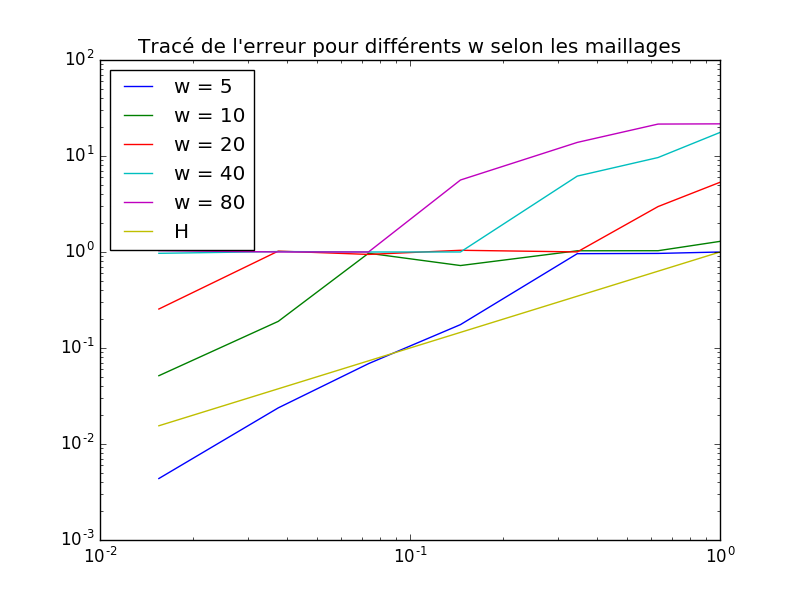
\includegraphics[width=225pt,height=225pt]{image/figure_1}
\end{center}
\caption{Caract\'eristiques dans le plan $(x,t)$ pour $a(x)=x$ et $a(x)=-x$}
\label{Caract\'eristiques dans le plan $(x,t)$ pour $a(x)=x$ et $a(x)=-x$}
\end{figure}

Par le calcul, on a les expressions des caract\'eristiques suivantes :\\
	\begin{itemize}
		\item Pour le cas avec $a(x)=x$ :\\
	    \begin{equation}
			  X_{x_0}(t)=x_0\exp(t)
			  \label{eq_1}
			\end{equation}
	  \item Pour le cas avec $a(x)=-x$ :\\
		  \begin{equation}
	      X_{x_0}(t)=x_0\exp(-t)
				\label{eq_2}
			\end{equation}
	\end{itemize}

Dans le cas o\`u $a(x)=x$, le terme $\exp(t)$ va entra\^iner une diffusion en temps croissant, c'est ce que l'on observe sur le graphe gauche de la Figure 1.\\
\tab \tab Dans le cas o\`u $a(x)=-x$, le terme $\exp(-t)$ va entra\^iner une contraction en temps croissant, c'est ce que l'on observe sur le graphe droit de la Figure 1.

\subsection{Question 2}

On utilise le calcul des caract\'eristiques fait pr\'ecedemment pour calculer la solution exacte en fonction de $u_{ini}$.
Ce qui donne pour solution dans le cas non-conservatif :
\begin{itemize}
  \item Pour $a(x)=x$ :\\
    \begin{equation}
		  \overline{u}(x,t)=u_{ini}(x\exp(-t))
			\label{eq_3}
		\end{equation}
	\item Pour $a(x)=-x$ :\\
	  \begin{equation}
		  \overline{u}(x,t)=u_{ini}(x\exp(t))
			\label{eq_4}
		\end{equation}
\end{itemize}
Dans le cas conservatif :\\
\begin{itemize}
  \item Pour $a(x)=x$ :\\
	  \begin{equation}
		  \hat{u}(x,t)=u_{ini}(x\exp(-t))\exp(-t)
			\label{eq_5}
		\end{equation}
	\item Pour $a(x)=-x$ :\\
	  \begin{equation}
		  \hat{u}(x,t)=u_{ini}(x\exp(t))\exp(t)
			\label{eq_6}
		\end{equation}
\end{itemize}
	
\subsection{Question 3}

Le sch\'ema $(6)$ peut se r\'e\'ecrire :\\
\[u_{j}^{n+1}=\alpha_j u_{j}^{n}+\beta_j u_{j-1}^{n}+\gamma_j u_{j+1}^{n}\]
\begin{center}
  o\`u $\left\{
	\begin{array}{r c l}
	\alpha_j&=&1-\frac{\Delta t}{\Delta x}(a_{j}^{+}+a_{j-1}^{-})\\
	\beta_j&=&\frac{\Delta t}{\Delta x}a_{j-1}^{+}\\
	\gamma_j&=&\frac{\Delta t}{\Delta x}a_{j}^{-}
	\end{array}
	\right.
	$
\end{center}
\'Etant donn\'e que $u_{j}^{n}$, $u_{j-1}^{n}$, $u_{j+1}^{n}$, $\beta_j$ et $\gamma_j$ sont positifs, et au vu de la r\'e\'ecriture du sch\'ema, pour que $u_{j}^{n+1}$ soit positif, il suffit que :
\begin{center}
  $\alpha_j \geq 0
	\iff \frac{\Delta t}{\Delta x}(a_{j}^{+}+a_{j-1}^{-}) \leq 1$
\end{center}
Et donc si $A$ est une borne de $a$, il suffit que :
\begin{equation}
  \frac{\Delta t}{\Delta x}2A \leq 1
	\label{eq_7}
\end{equation}
C'est notre condition CFL.

\subsection{Question 4}

Sous cette condition CFL, on a pour $k \in \mathbb{N}$ :
\[\sum_{j=-k}^{k} |u_{j}^{n+1}|=\sum_{j=-k}^{k} |\alpha_j u_{j}^{n}+\beta_j u_{j-1}^{n}+\gamma_j u_{j+1}^{n}|\]
Par in\'egalit\'e triangulaire :
\[\sum_{j=-k}^{k} |u_{j}^{n+1}| \leq \sum_{j=-k}^{k} \alpha_j u_{j}^{n}+\beta_j u_{j-1}^{n}+\gamma_j u_{j+1}^{n}\]
Or on a les in\'egalit\'es imm\'ediates suivantes :
\[
\left\{
\begin{array}{r c l}
\alpha_j \leq 1\\
\beta_j \leq \frac{\Delta t}{\Delta x}A\\
\gamma_j \leq \frac{\Delta t}{\Delta x}A
\end{array}
\right.
\]
On obtient donc que :
\[\sum_{j=-k}^{k} |u_{j}^{n+1}| \leq \sum_{j=-k}^{k} u_{j}^{n} +\frac{\Delta t}{\Delta x}A\left(\sum_{j=-k}^{k} u_{j-1}^{n} + \sum_{j=-k}^{k} u_{j+1}^{n}\right)\]
Or sous la condition CFL, on a :
\[\sum_{j\in\mathbb{Z}} |u_{j}^{n}|=\sum_{j\in\mathbb{Z}} u_{j}^{n}=\sum_{j\in\mathbb{Z}} u_{j-1}^{n}=\sum_{j\in\mathbb{Z}} u_{j+1}^{n}\]
On obtient alors :
\[\sum_{j=-k}^{k} |u_{j}^{n+1}| \leq \sum_{j\in\mathbb{Z}} u_{j}^{n} + \frac{\Delta t}{\Delta x}A\left(\sum_{j\in\mathbb{Z}} u_{j-1}^{n}+\sum_{j\in\mathbb{Z}} u_{j+1}^{n}\right)\]
\[\iff \sum_{j=-k}^{k} |u_{j}^{n+1}| \leq \left(1+2\frac{\Delta t}{\Delta x}A\right)\sum_{j\in\mathbb{Z}} u_{j}^{n}<+\infty\]
Et la s\'erie $\sum_{j\in\mathbb{Z}} |u_{j}^{n+1}|$ est \'egalement convergente, et par la m\^eme, la s\'erie $\sum_{j\in\mathbb{Z}} u_{j}^{n+1}$ est convergente. On a alors :
\[\sum_{j\in\mathbb{Z}} u_{j}^{n+1}=\sum_{j\in\mathbb{Z}} \alpha_j u_{j}^{n}+\beta_j u_{j-1}^{n}+\gamma_j u_{j+1}^{n}=\sum_{j\in\mathbb{Z}} (\alpha_j+\beta_{j+1}+\gamma_{j-1})u_{j}^{n}\]
Or pour $j\in\mathbb{Z}$ :
\[\alpha_j+\beta_{j+1}+\gamma_{j-1}=1\]
Et on a bien conservation de la masse discr\`ete :
\[\sum_{j\in\mathbb{Z}} \Delta x u_{j}^{n}=\sum_{j\in\mathbb{Z}} \Delta x u_{j}^{n+1}\]

\subsection{Question 5}

En utilisant les formules $a_j=a_{j}^{+}-a_{j}^{-}$ et $a_{j-1}=a_{j-1}^{+}-a_{j-1}^{-}$, puis en simplifiant les termes et en factorisant par $a_{j}^{-}$ et $a_{j-1}^{+}$, on obtient le r\'esultat.

\subsection{Question 6}

Ici, on peut r\'e\'ecrire le sch\'ema $(7)$ sous la forme :
\[u_{j}^{n+1}=H(u_{j}^{n},u_{j-1}^{n},u_{j+1}^{n}) \text{ , o\`u }
H:\begin{array}{ccccc}
\mathbb{R}^{3} & \to & \mathbb{R}\\
(u,v,w) & \mapsto & \alpha_{j} u + \beta_{j} v + \gamma_{j} w\\
\end{array}
\]
Avec :
\[\left\{\begin{array}{ccccc}
\alpha_{j}=1+\frac{\Delta t}{\Delta x}(a_{j}^{-}-a_{j-1}^{+})\\
\beta_{j}=\frac{\Delta t}{\Delta x}a_{j-1}^{+}\\
\gamma_{j}=-\frac{\Delta t}{\Delta x}a_{j}^{-}\\
\end{array}
\right.
\]
Donc le sch\'ema est associ\'e \`a un flux num\'erique lin\'eaire, qui est consistant si et seulement si $\forall u \in \mathbb{R}$, $H(u,u,u)=u$, i.e. si et seulement si $\forall j \in \mathbb{Z}$, $\alpha_{j} + \beta_{j} + \gamma_{j} = 1$. Et si de plus $\forall j \in \mathbb{Z}$, $\alpha_{j} \geq 0$, $\beta_{j} \geq 0$, $\gamma_{j} \geq 0$ alors $u_{j}^{n+1}=H(u_{j}^{n},u_{j-1}^{n},u_{j+1}^{n})$ est une combinaison lin\'eaire convexe et donc :
\[\forall j \in \mathbb{Z} \text{, } min(u_{j-1}^{n},u_{j}^{n},u_{j+1}^{n}) \leq u_{j}^{n+1} \leq max(u_{j-1}^{n},u_{j}^{n},u_{j+1}^{n})\]
Et par suite, on a :
\[\underset{j \in \mathbb{Z}}{min}(u_{j}^{0}) \leq u_{j}^{n} \leq \underset{j \in \mathbb{Z}}{max}(u_{j}^{0})\]
Ce qui implique la stabilit\'e $L^{\infty}$.
Ainsi, pour que le sch\'ema verifie le principe du maximum discret, il suffit que :
\[
\forall j \in \mathbb{Z} \text{, }
\left\{\begin{array}{ccccc}
\alpha_{j} + \beta_{j} + \gamma_{j} = 1\\
\alpha_{j} \geq 0\\
\beta_{j} \geq 0\\
\gamma_{j} \geq 0\\
\end{array}
\right.
\]
Or toutes ces conditions sont d\'ej\`a v\'erifi\'ees sauf $\alpha_{j} \geq 0$. Ce qui permet d'avoir notre condition CFL :
\[\alpha_{j} \geq 0\]
\[\iff \frac{\Delta t}{\Delta x}(a_{j-1}^{+}-a_{j}^{-}) \leq 1\]
Donc si :
\[2A\frac{\Delta t}{\Delta x} \leq 1\]
On a :
\[\frac{\Delta t}{\Delta x}(a_{j-1}^{+}-a_{j}^{-}) \leq \frac{\Delta t}{\Delta x}(a_{j-1}^{+}+a_{j}^{-}) \leq 2A\frac{\Delta t}{\Delta x} \leq 1\]
Donc notre condition CFL pour que le sch\'ema v\'erifie le principe du maximum discret et soit alors stable $L^{\infty}$ est la condition~\eqref{eq_7}.

\subsection{Question 8}

Tra\c{c}ons, pour diff\'erents temps $t$ dans la subdivision de $[0,T]$, la solution approch\'ee par le sch\'ema conservatif $(6)$ et la solution exacte donn\'ees par la fonction :
\begin{center}
  $u(.,t):\begin{array}{ccccc}
	[-2,2] & \to & \mathbb{R}\\
	x & \mapsto & u(x,t)\\
	\end{array}$
\end{center}
On obtient alors la figure 2.

\begin{figure}[h!]
\begin{center}
	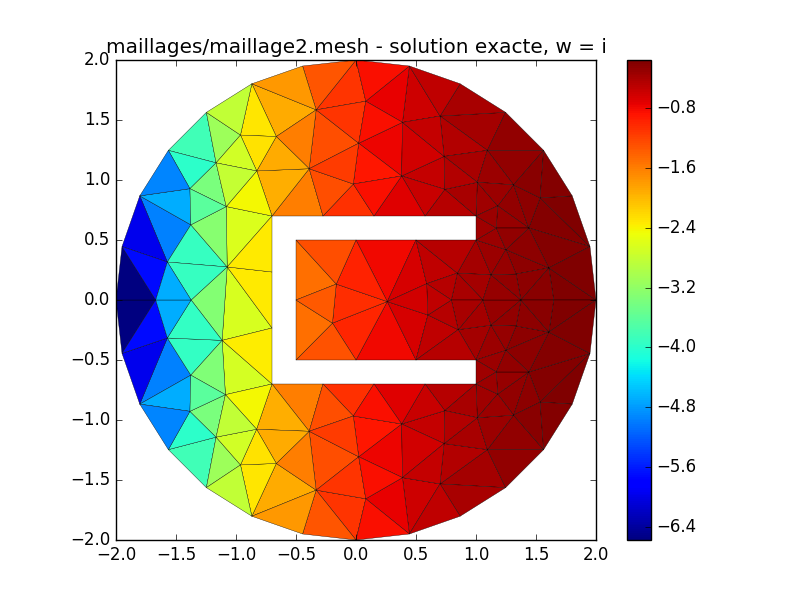
\includegraphics[width=225pt,height=225pt]{image/figure_2}
	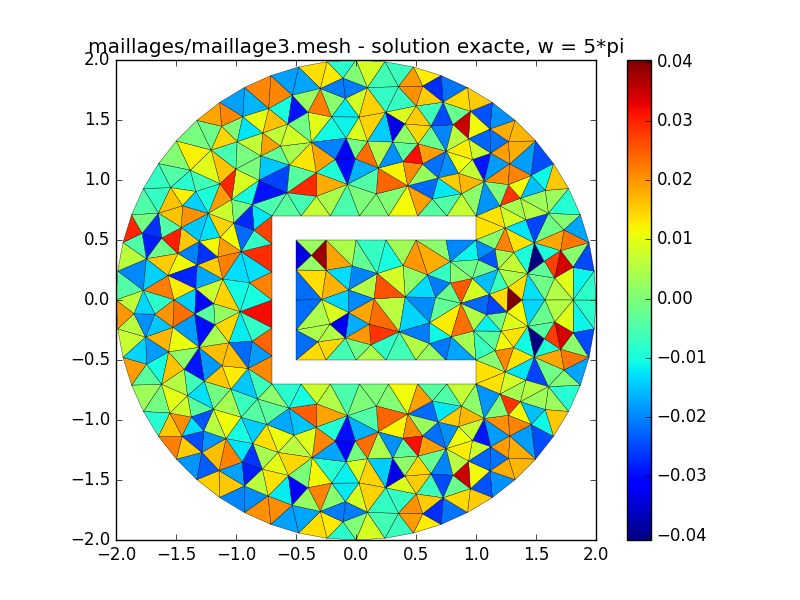
\includegraphics[width=225pt,height=225pt]{image/figure_3}
\end{center}
\caption{Solution exacte et approch\'ee dans le cas conservatif pour $a(x)=x$ et $a(x)=-x$}
\label{Solution exacte et approch\'ee dans le cas conservatif pour $a(x)=x$ et $a(x)=-x$}
\end{figure}

Dans le graphique de gauche, le cas o\`u $a(x)=x$, la solution exacte est :
\[\hat{u}(x,t)=u_{ini}(x\exp(-t))\exp(-t)=\left\{\begin{array}{ccccc}
\exp(-t) & \text{ , si }-\frac{1}{2} \leq x\exp(-t) \leq \frac{1}{2}\\
0 & \text{ , sinon}\\
\end{array}
\right.
\]
Donc lorsque $t$ augmente, $\exp(-t)$ diminue, ce qui fait que l'ensemble $\{x\in[-2,2] | -\frac{1}{2} \leq x\exp(-t) \leq \frac{1}{2}\}$ grandit. Ceci explique le graphique que l'on obtient, la "boite" rouge baisse en $\exp(-t)$ et s'\'elargit en $\exp(t)$, ce qui ne change rien pour l'aire dans cette "boite" et qui traduit le fait que l'\'equation soit conservative.\\

Dans le graphique de droite, le cas o\`u $a(x)=-x$, la solution exacte est :
\[\hat{u}(x,t)=u_{ini}(x\exp(t))\exp(t)=\left\{\begin{array}{ccccc}
\exp(t) & \text{ , si }-\frac{1}{2} \leq x\exp(t) \leq \frac{1}{2}\\
0 & \text{ , sinon}\\
\end{array}
\right.
\]
Donc lorsque $t$ augmente, $\exp(t)$ augmente, ce qui fait que l'ensemble $\{x\in[-2,2] | -\frac{1}{2} \leq x\exp(-t) \leq \frac{1}{2}\}$ diminue. Ceci explique le graphique que l'on obtient, la "boite" rouge monte en $\exp(t)$ et s'ammin\c{c}it en $\exp(-t)$, ce qui ne change rien pour l'aire dans cette "boite" et qui traduit encore le fait que l'\'equation soit conservative.

\subsection{Question 10}

Faisons de m\^eme pour le sch\'ema $(7)$ non-conservatif. On obtient la figure 3.\\
Rappelons l'expression de la solution exacte :\\
\begin{itemize}
\item Pour le cas $a(x)=x$ :
\[\overline{u}(x,t)=u_{ini}(x\exp(-t))=\left\{\begin{array}{ccccc}
1 & \text{ , si} -\frac{1}{2} \leq x\exp(-t) \leq \frac{1}{2}\\
0 & \text{ , sinon}\\
\end{array}
\right.
\]
\item Pour le cas $a(x)=-x$ :
\[\overline{u}(x,t)=u_{ini}(x\exp(t))=\left\{\begin{array}{ccccc}
1 & \text{ , si} -\frac{1}{2} \leq x\exp(t) \leq \frac{1}{2}\\
0 & \text{ , sinon}\\
\end{array}
\right.
\]
\end{itemize}
On a alors le m\^eme comportement pour la largeur des "boites", mais pas pour la hauteur. En effet, la valeur $1$ n'\'etant pas corrig\'ee pour conserver l'aire sous la courbe, le sch\'ema n'est pas conservatif.

\begin{figure}[h!]
\begin{center}
	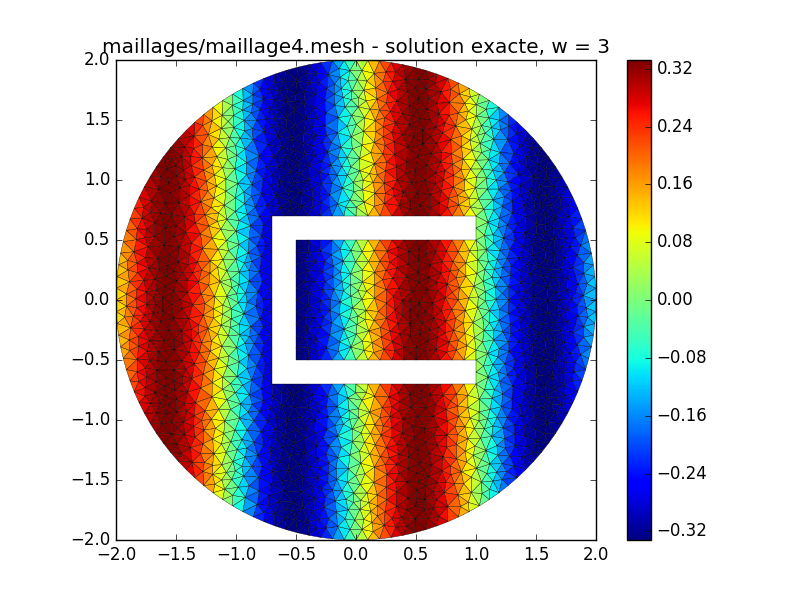
\includegraphics[width=225pt,height=225pt]{image/figure_4}
	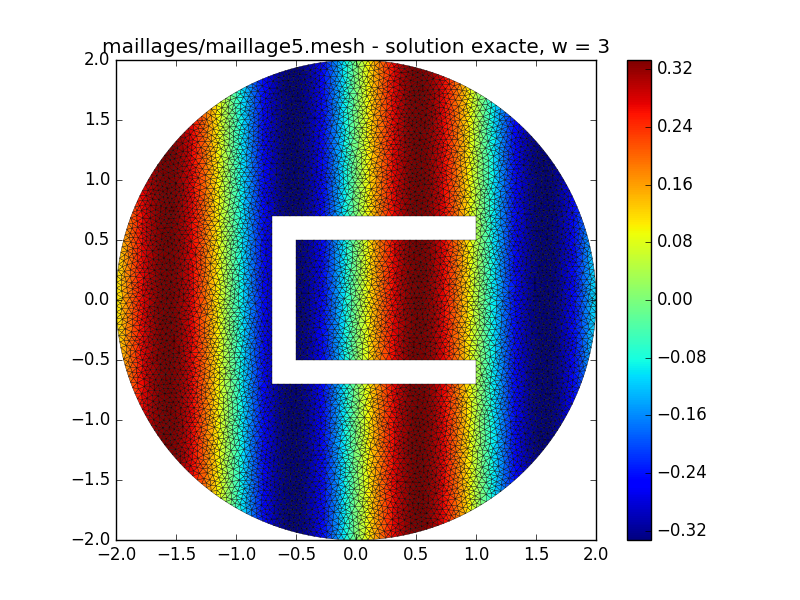
\includegraphics[width=225pt,height=225pt]{image/figure_5}
\end{center}
\caption{Solution exacte et approch\'ee dans le cas non-conservatif pour $a(x)=x$ et $a(x)=-x$}
\label{Solution exacte et approch\'ee dans le cas non-conservatif pour $a(x)=x$ et $a(x)=-x$}
\end{figure}

~
\newpage
~

\section{Probl\`eme stationnaire : \'el\'ements finis}

Pour plus de clart\'e et de l\'eg\`eret\'e, introduisons les notations suivantes :
\begin{itemize}
  \item $\Omega = ]0,1[$ et donc $\overline{\Omega}=[0,1]$.
	\item $\|.\|_{1,\Omega}$ designera la norme associ\'ee au produit scalaire suivant :
	  \begin{center}
		  $\langle .,. \rangle :\begin{array}{ccccc}
      H_{0}^{1}(\Omega)^{2} & \to & \mathbb{R} \\
      (u,v) & \mapsto & \int_{0}^{1} {u^{'}(x)v^{'}(x)+u(x)v(x) dx} \\
      \end{array}$
		\end{center}
	\item On d\'esigne par $a$ la forme bilin\'eaire sym\'etrique suivante :
	  \begin{center}
		  $a :\begin{array}{ccccc}
      H_{0}^{1}(\Omega)^{2} & \to & \mathbb{R} \\
      (u,v) & \mapsto & \int_{0}^{1} {u^{'}(x)v^{'}(x)+\lambda u(x)v(x) dx} \\
      \end{array}$
		\end{center}
	\item Et par $l$ la forme lin\'eaire suivante :
	  \begin{center}
		  $l :\begin{array}{ccccc}
      H_{0}^{1}(\Omega) & \to & \mathbb{R} \\
      v & \mapsto & \int_{0}^{1} {f(x)v(x) dx} \\
      \end{array}$
		\end{center}
\end{itemize}

\subsection{Question 1}

On applique le th\'ero\`eme de Lax-Milgram au probl\`eme variationnel $(FV_D)$ :

\begin{itemize}
  \item $H_{0}^{1}(\Omega)$ muni de la norme $\|.\|_{1,\Omega}$ est un espace de Hilbert.
	\item La forme bilin\'eaire $a$ est continue :\\
Soient $u,v$ dans $H_{0}^{1}(\Omega)$,
\begin{center}
  $|a(u,v)| \leq \int_{0}^{1} {|u^{'}(x)||v^{'}(x)| dx}+|\lambda|\int_{0}^{1} {|u(x)||v(x)| dx} \text{ , par l'in\'egalit\'e triangulaire}$
	$|a(u,v)| \leq \|u^{'}\|_{L^{2}}\|v^{'}\|_{L^{2}}+|\lambda|\|u\|_{L^{2}}\|v\|_{L^{2}} \text{ , par l'in\'egalit\'e de Cauchy-Schwartz}$
\end{center}
d'o\`u,
	\[|a(u,v)| \leq \|u\|_{1,\Omega}\|v\|_{1,\Omega}(1+|\lambda|)\]
et $a$ est continue.
  \item $a$ est coercive :\\
Soit $u$ dans $H_{0}^{1}(\Omega)$,
\[a(u,u)=\int_{0}^{1} {u'(x)^{2}+\lambda u^{2}(x) dx}=\int_{0}^{1} {u'(x)^{2} dx}+\lambda\int_{0}^{1} {u^{2}(x) dx}\]
\[a(u,u)=\lambda \|u\|_{1,\Omega}^{2}+(1-\lambda)\int_{0}^{1}{u'(x)^{2} dx}\]
Or d'apr\'es l'in\'egalit\'e d'Henri Poincar\'e :\\
\[\exists \beta > 0 \text{ , } \int_{0}^{1}{u'(x)^{2} dx} \geq \beta\int_{0}^{1}{u(x)^{2} dx}\]
donc :
\[(1-\lambda)\int_{0}^{1}{u'(x)^{2} dx} = \frac{1-\lambda}{2}\int_{0}^{1}{u'(x)^{2} dx}+\frac{1-\lambda}{2}\int_{0}^{1}{u'(x)^{2} dx}\]
\[(1-\lambda)\int_{0}^{1}{u'(x)^{2} dx} \geq \frac{1-\lambda}{2}\int_{0}^{1}{u'(x)^{2} dx}+\frac{(1-\lambda)\beta}{2}\int_{0}^{1}{u(x)^{2} dx}\]
D'o\`u,
\[a(u,u) \geq \left(\lambda+\frac{1-\lambda}{2}min(1,\beta)\right)\|u\|_{1,\Omega}^{2}\]
et $a$ est coercive.
  \item La forme lin\'eaire $l$ est continue :\\
	Soit $v$ dans $H_{0}^{1}(\Omega)$,
	\[|l(v)| \leq \int_{0}^{1} {|f(x)||v(x)| dx}\]
	\[|l(v)| \leq \|f\|_{L^{2}}\|v\|_{L^{2}}\]
	\[|l(v)| \leq \|f\|_{L^{2}}\|v\|_{1,\Omega}\]
et $l$ est continue.
\end{itemize}
Ainsi, d'apr\`es le th\'eor\`eme de Lax-Milgram, il y a existence et unicit\'e de la solution au probl\`eme variationnel $(FV_{D})$.\\
On sait que les probl\`emes $(D)$ et $(FV_D)$ sont \'equivalents, donc pour v\'erifier que $u(x)=\sin(\pi x)$ est solution faible de $(FV_D)$ avec pour second membre $f(x)=(1+\pi^{2})\sin(\pi x)$, il suffit de v\'erifier qu'elle est solution de $(D)$. Et en effet, on a :
\[u(0)=\sin(0)=u(1)=\sin(\pi)=0\]
Et on a les d\'eriv\'ees premi\`ere et seconde de $u$ suivantes :
\[\left\{\begin{array}{ccccc}
u^{'}(x)&=&\pi\cos(\pi x) &\\
u^{''}(x)&=&-\pi^{2}\sin(\pi x) & =-\pi^{2}u(x)\\
\end{array}
\right.
\]
Et donc pour $\lambda=1$, on a :
\[-u^{''}(x)+u(x)=\pi^{2}\sin(\pi x)+\sin(\pi x)=(1+\pi^{2})\sin(\pi x)=f(x)\]
Ainsi, $u$ est solution de $(D)$ et donc de $(FV_D)$.

\subsection{Question 2}

Avec les notations introduites, et en remarquant que $u_h=\sum_{k=1}^{N} u_h(x_k) \varphi_{h,k}$, le probl\`eme $(EF_D)$ se r\'e\'ecrit :
\[(EF_D)\left\{\begin{array}{ccccc}
\text{Trouver } u_h \in V_{h}^{1} \text{ telle que, pour tout } j=1,...,N\text{, on ait :}\\
a(u_h,\varphi_{h,j})=l(\varphi_{h,j})\\
\end{array}
\right.
\]
Or :
\[a(u_h,\varphi_{h,j})=a\left(\sum_{k=1}^{N} u_h(x_k) \varphi_{h,k},\varphi_{h,j}\right)=\sum_{k=1}^{N} u_h(x_k) a(\varphi_{h,k},\varphi_{h,j})
\]
Donc $\tilde{u}_{h}=(u_h(x_1),...,u_h(x_N))^t$ est solution du syst\`eme lin\'eaire suivant :
\begin{equation}
  A_{h}\tilde{u}_{h}=b_{h}
	\label{eq_8}
\end{equation}
O\`u,
\[A_h=(a(\varphi_{h,k},\varphi_{h,j})_{1 \leq k,j \leq N}\]
\[b_h=(l(\varphi_{h,j}))_{1 \leq j \leq N}\]
Calculons d\'esormais les coefficients de la matrice $A_h$. Donnons tout d'abord une expression claire des \'el\'ements de la base de $V_{1}^{h}$ :
\[\forall k \in \{1,...,N\}, \forall x \in [0,1], \varphi_{h,k}(x)=\left\{\begin{array}{ccccc}
&\frac{x-x_{k-1}}{h}& \text{ , si } x \in [x_{k-1},x_k]\\
&\frac{x_{k+1}-x}{h}& \text{ , si } x \in [x_k,x_{k+1}]\\
&0& \text{ , sinon}\\
\end{array}
\right.
\]
D\`es lors, le support d'un $\varphi_{h,k}$ ou de sa d\'eriv\'ee est $[x_{k-1},x_{k+1}]$. Ainsi, les produits $\varphi_{h,k}\varphi_{h,j}$ et $\varphi'_{h,k}\varphi'_{h,j}$ sont nuls sur $[0,1]$ d\`es que $|k-j|\geq 2$, ce qui fait de $A_h$ une matrice tridiagonale. Par ailleurs la forme bilin\'eaire $a$ est sym\'etrique, donc la sous diagonale et la sur diagonale de $A_h$ sont identiques au d\'ecalage d'indice pr\`es. Il nous reste donc plus que deux calculs \`a faire pour expliciter toute la matrice $A_h$ : celui de $a(\varphi_{h,k},\varphi_{h,k-1})$ et $a(\varphi_{h,k},\varphi_{h,k})$.
\[a(\varphi_{h,k},\varphi_{h,k-1})=\int_{0}^{1} {\varphi_{h,k}^{'}(x)\varphi_{h,k-1}^{'}(x)+\lambda\varphi_{h,k}(x)\varphi_{h,k-1}(x) dx}\]
\[=\int_{x_{k-1}}^{x_k} {\varphi_{h,k}^{'}(x)\varphi_{h,k-1}^{'}(x)+\lambda\varphi_{h,k}(x)\varphi_{h,k-1}(x) dx}\]
\[=-\frac{1}{h}+\lambda\int_{x_{k-1}}^{x_k} {\frac{x-x_{k-1}}{x_k-x_{k-1}}\frac{x_k-x}{x_k-x_{k-1}} dx}\]
\[=-\frac{1}{h}+\frac{\lambda}{h^2}\int_{x_{k-1}}^{x_k} {(x-x_k+x_k-x_{k-1})(x_k-x) dx}\]
\[=-\frac{1}{h}+\frac{\lambda}{h^2}\int_{x_{k-1}}^{x_k} {-(x-x_k)^{2}+h(x_k-x) dx}\]
\[=-\frac{1}{h}-\frac{\lambda}{h^2}\left[\frac{(x-x_k)^{3}}{3}\right]_{x_{k-1}}^{x_k}+\frac{\lambda}{h}\left[\frac{(x_k-x)^{2}}{-2}\right]_{x_{k-1}}^{x_k}\]
\[=-\frac{1}{h}-\frac{\lambda}{h^2}\frac{h^{3}}{3}+\frac{\lambda}{h}\frac{h^{2}}{2}\]
\[=-\frac{1}{h}-\frac{\lambda h}{3}+\frac{\lambda h}{2}\]
\[a(\varphi_{h,k},\varphi_{h,k-1})=-\frac{1}{h}+\frac{\lambda h}{6}\]
Et :
\[a(\varphi_{h,k},\varphi_{h,k})=\int_{0}^{1} {\varphi_{h,k}^{'}(x)^{2}+\lambda\varphi_{h,k}(x)^{2} dx}\]
\[=\int_{x_{k-1}}^{x_k} {\varphi_{h,k}^{'}(x)^{2} dx}+\lambda\int_{x_{k-1}}^{x_k} {\varphi_{h,k}(x)^{2} dx}+\int_{x_{k}}^{x_{k+1}} {\varphi_{h,k}^{'}(x)^{2} dx}+\lambda\int_{x_{k}}^{x_{k+1}} {\varphi_{h,k}(x)^{2} dx}\]
\[=\frac{2}{h}+\lambda\int_{x_{k-1}}^{x_k} {\left(\frac{x-x_{k-1}}{h}\right)^{2} dx}+\lambda\int_{x_k}^{x_{k+1}} {\left(\frac{x_{k+1}-x}{h}\right)^{2} dx}\]
\[=\frac{2}{h}+\frac{\lambda}{h^2}\left(\left[\frac{(x-x_{k-1})^{3}}{3}\right]_{x_{k-1}}^{x_k}+\left[\frac{(x_{k+1}-x)^{3}}{-3}\right]_{x_{k}}^{x_{k+1}}\right)\]
\[=\frac{2}{h}+\frac{\lambda}{h^2}(\frac{2h^{3}}{3})\]
\[=\frac{2}{h}+\frac{2h\lambda}{3}\]
On a donc les coefficients de la matrice $A_h$. Calculons d\'esormais les coefficients de $b_h$, i.e. $l(\varphi_{h,k})$ pour $k=\{1,...,N\}$ :
\[l(\varphi_{h,k})=\int_{0}^{1}{f(x)\varphi_{h,k}(x) dx}\]
\[=\int_{x_{k-1}}^{x_k}{(1+\pi^{2})\sin(\pi x)\left(\frac{x-x_{k-1}}{x_k-x{k-1}}\right) dx}+\int_{x_k}^{x_{k+1}}{(1+\pi^{2})\sin(\pi x)\left(\frac{x_{k+1}-x}{x_{k+1}-x_k}\right) dx}\]
\[=\frac{1+\pi^2}{h}\left(\int_{x_{k-1}}^{x_k}{\sin(\pi x)(x-x_{k-1}) dx}+\int_{x_k}^{x_{k+1}}{\sin(\pi x)(x_{k+1}-x) dx}\right)\]
Et en int\'egrant par partie, on obtient :
\[l(\varphi_{h,k})=\frac{1+\pi^2}{h}\left(\left[-\frac{\cos(\pi x)}{\pi}(x-x_{k-1})\right]_{x_{k-1}}^{x_k}+\frac{1}{\pi}\int_{x_{k-1}}^{x_k}{\cos(\pi x) dx}+\left[-\frac{\cos(\pi x)}{\pi}(x_{k+1}-x)\right]_{x_{k}}^{x_{k+1}}\right.\]
\[\left. -\frac{1}{\pi}\int_{x_{k}}^{x_{k+1}}{\cos(\pi x) dx}\right)\]
\[=\frac{1+\pi^2}{h}\left(\frac{1}{\pi}\int_{x_{k-1}}^{x_k}{\cos(\pi x) dx}-\frac{1}{\pi}\int_{x_{k}}^{x_{k+1}}{\cos(\pi x) dx}\right)\]
\[=\frac{1+\pi^2}{h\pi}\left(\left[\frac{\sin(\pi x)}{\pi}\right]_{x_{k-1}}^{x_k}-\left[\frac{\sin(\pi x)}{\pi}\right]_{x_k}^{x_{k+1}}\right)\]
\[=\frac{1+\pi^2}{h\pi^2}(2\sin(\pi x_k)-\sin(\pi x_{k+1})-\sin(\pi x_{k-1}))\]
Et en utilisant la formule trigonom\'etrique $\sin(p)+\sin(q)=2\sin(\frac{p+q}{2})\cos(\frac{p-q}{2})$ pour $p=\pi x_{k+1}$ et $q=\pi x_{k-1}$, on obtient :
\[\sin(\pi x_{k+1})+\sin(\pi x_{k-1})=2\sin(\pi x_k)\cos(\pi h)\]
Et donc :
\[l(\varphi_{h,k})=\frac{1+\pi^2}{h\pi^2}2\sin(\pi x_k)(1-\cos(\pi h))\]

\subsection{Question 4}

Tra\c{c}ons pour N variant dans $\{5, 10, 25, 50, 100\}$, le graphique de la solution exacte et de la solution approch\'ee. On obtient alors la figure 3.

\begin{figure}[h!]
\begin{center}
	\includegraphics[width=225pt,height=200pt]{image/figure_10}
	\includegraphics[width=225pt,height=200pt]{image/figure_9}
	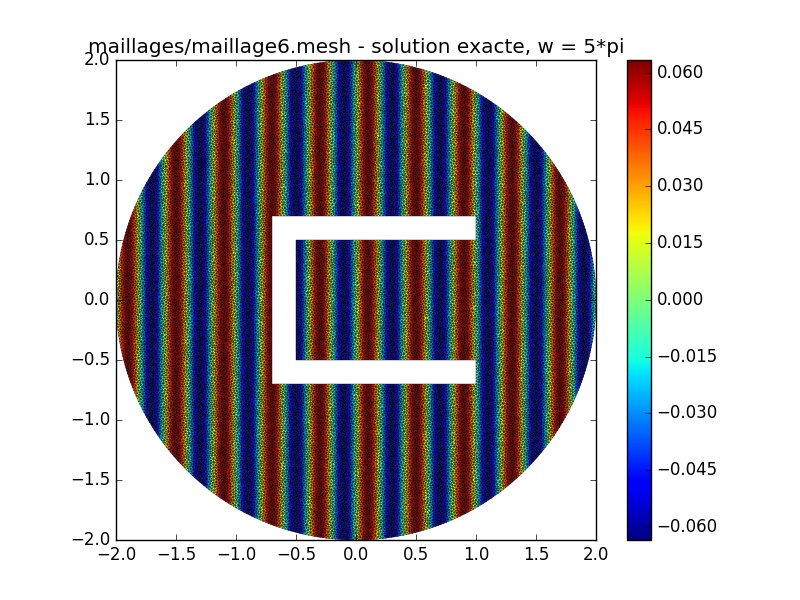
\includegraphics[width=225pt,height=200pt]{image/figure_6}
  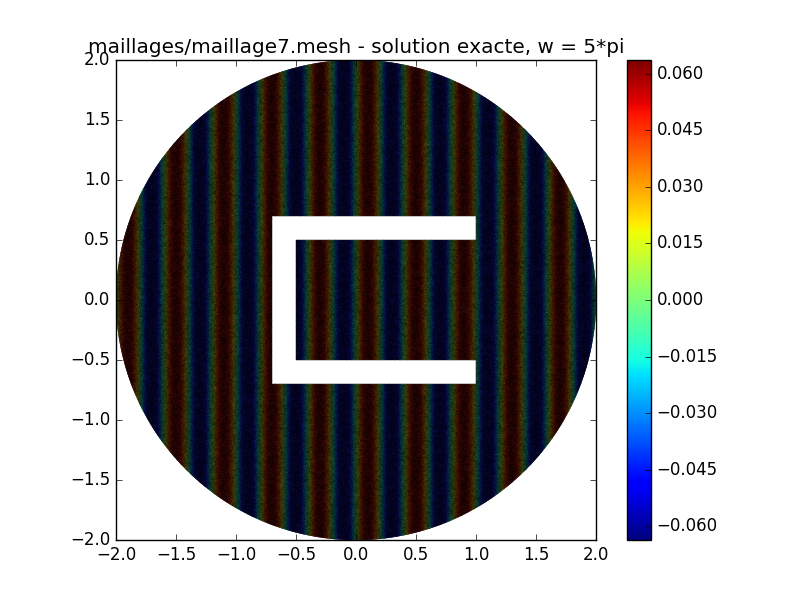
\includegraphics[width=225pt,height=200pt]{image/figure_7}
  \includegraphics[width=225pt,height=200pt]{image/figure_8}
\end{center}
\caption{Solution exacte et approch\'ee pour diff\'erentes valeurs de N}
\label{Solution exacte et approch\'ee pour diff\'erentes valeurs de N}
\end{figure}

On voit alors que la m\'ethode des \'el\'ements finis est tr\`es \'efficace, graphiquement au premier coup d'oeil on pourrait se demander si la m\'ethode n'est pas exacte. Mais on voit ici que pour $N=5$, la solution approch\'ee est leg\`erement au-dessus de $1$.

\subsection{Question 5}

Pour comparer graphiquement les d\'eriv\'ees de notre solution exacte et notre solution approch\'ee, il faut se demander de quelle d\'eriv\'ee on vas parler. La solution exacte est $u(x)=\sin(\pi x)$ qui est une fonction de $C^{\infty}(\Omega)$, et donc on parle de sa d\'eriv\'ee forte qui coincide avec sa d\'eriv\'ee faible. Concernant la solution approch\'ee qui est donn\'ee par $u_{h}=\sum_{k=1}^{N} u_{h}(x_{k})\phi_{h,k}$ qui seulement dans $C^{0}(\Omega)$, on d\'efinit sa d\'eriv\'ee faible sur $\Omega$ par la d\'eriv\'ee forte de $u_{h}$ r\'estreinte aux sous intervalles $[x_{i},x_{i+1}]$. La fonction $u_h$ \'etant affine sur chacun de ces intervalles, la d\'eriv\'ee faible de $u_h$ sur $\Omega$ est en fait une fonction constante par morceaux discontinue. Le petit calcul suivant peut nous en convaincre :\\
Soit $k \in \{0,...N\}$,
\[u_{h|[x_{k},x_{k+1}]}(t)=u_{h}(x_{k})\frac{t-x_{k+1}}{x_{k}-x_{k+1}}+u_{h}(x_{k+1})\frac{t-x_{k}}{x_{k+1}-x_{k}}\]
\[u_{h|[x_{k},x_{k+1}]}(t)=\frac{1}{h}((u_{h}(x_{k+1})-u_{h}(x_{k}))t-u_{h}(x_{k})x_{k+1}-u_{h}(x_{k+1})x_{k})\]
Donc :
\begin{equation}
u_{h|[x_{k},x_{k+1}]}^{'}(t)=\frac{u_{h}(x_{k+1})-u_{h}(x_{k})}{h}
\label{eq_9}
\end{equation}
On peut alors calculer les d\'eriv\'ees voulues et les tra\c{c}er, ce  pour les m\^emes valeurs de $N$ qu'\`a la question pr\'ecedente. On obtient la figure 5.

\begin{figure}[h!]
\begin{center}
	\includegraphics[width=225pt,height=200pt]{image/figure_11}
	\includegraphics[width=225pt,height=200pt]{image/figure_12}
	\includegraphics[width=225pt,height=200pt]{image/figure_13}
  \includegraphics[width=225pt,height=200pt]{image/figure_14}
  \includegraphics[width=225pt,height=200pt]{image/figure_15}
\end{center}
\caption{D\'eriv\'ees de la solution exacte et approch\'ee pour diff\'erentes valeurs de N}
\label{D\'eriv\'ees de la solution exacte et approch\'ee pour diff\'erentes valeurs de N}
\end{figure}

On voit alors que pour la solution exacte, comme pour la solution approch\'ee, on obtient la fonction qu'il faut, i.e. :\\
\[u'(x)=\pi\cos(\pi x)\]
Autrement dit, que par la m\'ethode des \'el\'ements finis, la d\'eriv\'ee faible de notre solution approch\'ee approche la d\'eriv\'ee de notre solution exacte. Ce que l'on peut expliquer gr\^ace \`a~\eqref{eq_1}, en effet on y voit que si $N \to +\infty$, alors $h \to 0$ et~\eqref{eq_9} est en fait une limite de taux d'accroissement.

\subsection{Question 6}

Explicitons tout d'abord un petit calcul qui permet d'expliquer comment a \'et\'e cod\'e le calcul des normes.
\[\|u-u_{h}\|_{0}^{2}=\sum_{i=0}^{N} \int_{x_{i}}^{x_{i+1}}{(u-u_{h})^{2}(x) dx}\]
Qui s'approche par la m\'ethode des trap\`ezes par :\\
\[\|u-u_{h}\|_{0}^{2} \simeq \frac{h}{2} \sum_{i=0}^{N} ((u-u_{h})^{2}(x_{i+1})+(u-u_{h})^{2}(x_{i}))\]
Or le premier et dernier terme de cette somme sont nuls, et tous les autres apparaissent deux fois. On a donc :
\[\|u-u_{h}\|_{0}^{2} \simeq h \sum_{i=1}^{N} (u-u_{h})^{2}(x_{i})=h\|((u-u_{h})(x_{i}))_{1 \leq i \leq N}\|_{2}^{2}\]
Calculons \'egalement $|u-u_{h}|_{1}^{2}$ :
\[|u-u_{h}|_{1}^{2} = \int_{0}^{1}{\left(u'-u'_{h}\right)^{2}(x) dx}\]
\[|u-u_{h}|_{1}^{2} = \sum_{i=1}^{N+1} \int_{x_{i}}^{x_{i+1}}{\left(u'-u'_{h}\right)^{2}(x) dx}\]
Avec la formule~\eqref{eq_9}, $u'_{h}$ est constante sur $[x_{i},x_{i+1}]$, on notera donc seulement $u'_{h}$ sa valeur. On a alors :
\[\int_{x_{i}}^{x_{i+1}}{\left(u'-u'_{h}\right)^{2}(x) dx} = \int_{x_{i}}^{x_{i+1}}{\left(u'(x)^{2}-2u'(x)u'_{h}+{u'_{h}}^{2} \right) dx}\]
\[\int_{x_{i}}^{x_{i+1}}{\left(u'-u'_{h}\right)^{2}(x) dx} = \int_{x_{i}}^{x_{i+1}}{u'(x)^{2} dx}-2u'_{h}\int_{x_{i}}^{x_{i+1}}{u'(x) dx}+h{u'_{h}}^{2}\]
On approche le premier membre par le m\'ethodes des trap\`ezes :
\[\int_{x_{i}}^{x_{i+1}}{\left(u'-u'_{h}\right)^{2}(x) dx} = \frac{h}{2}(u'(x_{i+1})+u'(x_{i}))-\frac{2}{h}(u_h(x_{i+1})-u_h(x_{i}))(u(x_{i+1})-u(x_{i}))+\frac{1}{h}(u_h(x_{i+1})-u_h(x_{i}))^{2}\]
Et il ne reste plus qu'\`a faire la somme pour obtenir $|u-u_{h}|_{1}^{2}$.

\subsection{Question 7}

On calcul les erreurs en norme $0$ et $1$ gr\^ace aux calculs faits en question 6. Et asymptotiquement, on a :
\[\|u-u_{h}\|_{0} \simeq C_{1}h^{p_{1}} \text{ et } \|u-u_{h}\|_{1} \simeq C_{2}h^{p_{2}}\]
Donc :
\[\log(\|u-u_{h}\|_{0}) \simeq \log(C_{1})+p_{1}\log(h) \text{ et } \log(\|u-u_{h}\|_{1}) \simeq \log(C_{2})+p_{2}\log(h)\]
Donc pour deux pas de maillage $h_{1}$ et $h_{2}$, on a :
\[p_{1} \simeq \frac{\log(\|u-u_{h_{1}}\|_{0})-\log(\|u-u_{h_{2}}\|_{0})}{\log(h_{1})-\log(h_{2})} \text{ et } p_{2} \simeq \frac{\log(\|u-u_{h_{1}}\|_{1})-\log(\|u-u_{h_{2}}\|_{1})}{\log(h_{1})-\log(h_{2})}\]
On trouve alors num\'eriquement :
\[p_{1} \simeq 2 \text{ et } p_{2} \simeq 1\]

\end{document}

